\documentclass[12pt,a4paper]{article}
\usepackage[utf8]{vietnam}
\usepackage{amsmath,amssymb}
\usepackage{tabularx}
\usepackage{tikz}
\usetikzlibrary{calc,angles,quotes,arrows.meta,patterns}
\usepackage{xcolor}
\usepackage{enumitem}
\usepackage{fancyhdr}
\usepackage{graphicx}
\usepackage[top=0.9cm, bottom=0.9cm, left=1.2cm, right=1.2cm]{geometry}
\usepackage[sol]{ex_test}
\SAOPTN{widthSA=3.2,heightSA=0.62}

\setlength{\headheight}{15pt}
\setlength{\parskip}{0pt}

\pagestyle{fancy}
\fancyhf{}
\rhead{\textit{Hướng dẫn giải chi tiết -- Đề số 10}}
\lhead{\textit{Môn Toán 9 -- Giữa học kì I}}
\cfoot{\thepage}

\begin{document}

\begin{center}
  \textbf{\Large HƯỚNG DẪN GIẢI CHI TIẾT -- ĐỀ SỐ 10}\\
  \textbf{\large MÔN TOÁN 9 -- GIỮA HỌC KỲ I}
\end{center}
\vspace{2mm}

% --- BẢNG ĐÁP ÁN TỔNG HỢP ---
\noindent\textbf{\large I. BẢNG ĐÁP ÁN TỔNG HỢP}

\vspace{1mm}
\noindent\textbf{1. Phần I - Trắc nghiệm nhiều phương án lựa chọn (3,0 điểm):}
\begin{center}
\begin{tabular}{|c|c|c|c|c|c|c|c|c|c|c|c|c|}
\hline
\textbf{Câu} & \textbf{1} & \textbf{2} & \textbf{3} & \textbf{4} & \textbf{5} & \textbf{6} & \textbf{7} & \textbf{8} & \textbf{9} & \textbf{10} & \textbf{11} & \textbf{12} \\
\hline
\textbf{Chọn} & \textbf{C} & \textbf{C} & \textbf{D} & \textbf{C} & \textbf{C} & \textbf{A} & \textbf{A} & \textbf{C} & \textbf{D} & \textbf{C} & \textbf{B} & \textbf{A} \\
\hline
\end{tabular}
\end{center}
\vspace{1mm}

\noindent\textbf{2. Phần II - Trắc nghiệm Đúng/Sai (2,0 điểm):}
\begin{center}
\begin{tabular}{|c|c|c|c|c||c|c|c|c|c|}
\hline
\textbf{Câu} & \textbf{Lệnh hỏi} & \textbf{Đúng} & \textbf{Sai} & \textbf{Điểm} & \textbf{Câu} & \textbf{Lệnh hỏi} & \textbf{Đúng} & \textbf{Sai} & \textbf{Điểm} \\
\hline
 & a) & \textbf{X} & & 0,1 & & a) & \textbf{X} & & 0,1 \\
\cline{2-5}\cline{7-10}
\textbf{1} & b) & & \textbf{X} & 0,25 & \textbf{2} & b) & & \textbf{X} & 0,25 \\
\cline{2-5}\cline{7-10}
 & c) & \textbf{X} & & 0,5 & & c) & \textbf{X} & & 0,5 \\
\cline{2-5}\cline{7-10}
 & d) & \textbf{X} & & 1,0 & & d) & & \textbf{X} & 1,0 \\
\hline
\end{tabular}
\end{center}
\vspace{1mm}

\noindent\textbf{3. Phần III - Trả lời ngắn (1,0 điểm):}
\begin{center}
\begin{tabular}{|c|c|c|}
\hline
\textbf{Câu} & \textbf{1} & \textbf{2} \\
\hline
\textbf{Đáp án} & $\mathbf{x = 5}$ & $\mathbf{8\text{ cm}}$ \\
\hline
\end{tabular}
\end{center}
\vspace{3mm}

% --- LỜI GIẢI CHI TIẾT ---
\noindent\textbf{\large II. HƯỚNG DẪN GIẢI CHI TIẾT}

\vspace{2mm}
\noindent\textbf{\large PHẦN I. CÂU TRẮC NGHIỆM NHIỀU PHƯƠNG ÁN LỰA CHỌN}
\vspace{1mm}
\begin{ex}
Số nghiệm của phương trình $\left(x + \frac{1}{3}\right)(x - 3) = 0$ là:
\choice
{1}
{3}
{\True 2}
{Vô nghiệm}
\loigiai{
Phương trình tích $\left(x + \frac{1}{3}\right)(x - 3) = 0 \iff x + \frac{1}{3} = 0$ hoặc $x - 3 = 0 \iff x = -\frac{1}{3}$ hoặc $x = 3$. Phương trình có 2 nghiệm phân biệt.
}
\end{ex}

\begin{ex}
Bất phương trình $4x > 3x + 7$ có nghiệm là:
\choice
{$x > -7$}
{$x \le -7$}
{\True $x > 7$}
{$x < -7$}
\loigiai{
Chuyển vế và đổi dấu: $4x - 3x > 7 \iff x > 7$.
}
\end{ex}

\begin{ex}
Nghiệm của hệ phương trình $\begin{cases} x + y = 7 \\ x - y = -1 \end{cases}$ là:
\choice
{$(x; y) = (4; 3)$}
{$(x; y) = (5; 4)$}
{$(x; y) = (-3; 4)$}
{\True $(x; y) = (3; 4)$}
\loigiai{
Cộng hai phương trình vế theo vế: $2x = 6 \implies x = 3$. Thay vào phương trình đầu: $3 + y = 7 \implies y = 4$. Vậy nghiệm là $(3; 4)$.
}
\end{ex}

\begin{ex}
Nếu $a, b, c$ là ba số mà $a < b$ và $ac > bc$ thì $c$ là:
\choice
{Số 0}
{Số dương}
{\True Số âm}
{Số tùy ý}
\loigiai{
Khi nhân cả hai vế của bất đẳng thức $a < b$ với cùng một số $c$, chiều của bất đẳng thức bị đổi từ $<$ sang $>$ ($ac > bc$). Điều này xảy ra khi và chỉ khi $c$ là số âm ($c < 0$).
}
\end{ex}

\begin{ex}
Bất phương trình nào dưới đây là bất phương trình bậc nhất một ẩn?
\choice
{$\frac{1}{x} - 1 > 0$}
{$x^2 > 0$}
{\True $\frac{1}{3}x + 2 < 0$}
{$0 \cdot x + 3 > 0$}
\loigiai{
Bất phương trình bậc nhất một ẩn có dạng $ax + b < 0$ (hoặc $>$, $\le$, $\ge$) với $a \neq 0$. Biểu thức $\frac{1}{3}x + 2 < 0$ có $a = \frac{1}{3} \neq 0$ và ẩn $x$ bậc 1 nên là bất phương trình bậc nhất một ẩn.
}
\end{ex}

\begin{ex}
Những số nào sau đây là nghiệm của bất phương trình $2x - 10 < 0$?
\choice
{\True $-2; 0$}
{$0; 5$}
{$-2; 0; 5$}
{$-2; 4; 6$}
\loigiai{
Giải bất phương trình: $2x - 10 < 0 \iff 2x < 10 \iff x < 5$. Các số $-2$ và $0$ đều nhỏ hơn 5 nên thỏa mãn.
}
\end{ex}

\newpage
\begin{ex}
Cho tam giác $ABC$ vuông tại $A$, đường cao $AH$. Trong tam giác vuông $ABH$, $\cos B$ bằng:
\begin{center}
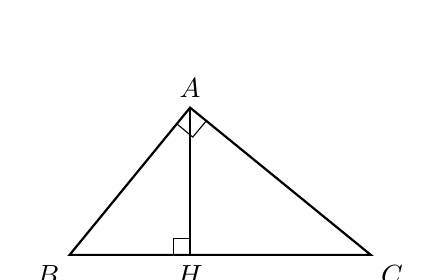
\begin{tikzpicture}[scale=0.85]
  \coordinate (B) at (0,0);
  \coordinate (H) at (1.8,0);
  \coordinate (C) at (4.5,0);
  \coordinate (A) at (1.8,2.2);
  \draw[thick] (B) node[below left]{$B$} -- (C) node[below right]{$C$} -- (A) node[above]{$A$} -- cycle;
  \draw[thick] (A) -- (H) node[below]{$H$};
  \draw (A) ++(-0.2,-0.24) -- ++(0.24,-0.2) -- ++(0.2,0.24);
  \draw (H) ++(0,0.25) -- ++(-0.25,0) -- ++(0,-0.25);
\end{tikzpicture}
\end{center}
\choice
{\True $\frac{BH}{AB}$}
{$\frac{AH}{AB}$}
{$\frac{BH}{AH}$}
{$\frac{AB}{AC}$}
\loigiai{
Xét tam giác $ABH$ vuông tại $H$, góc $B$ có cạnh kề là $BH$ và cạnh huyền là $AB$. Theo định nghĩa tỉ số lượng giác, $\cos B = \frac{BH}{AB}$.
}
\end{ex}

\begin{ex}
Cho tam giác $ABC$ vuông tại $A$, $AB = 4$ và $BC = 5$. Khẳng định nào sau đây là đúng?
\choice
{$\sin B = \frac{4}{5}$}
{$\cos B = \frac{3}{5}$}
{\True $\tan B = \frac{3}{4}$}
{$\cot B = \frac{3}{4}$}
\loigiai{
Áp dụng định lí Pythagore: $AC = \sqrt{BC^2 - AB^2} = \sqrt{5^2 - 4^2} = 3$. Đối với góc $B$, cạnh đối là $AC = 3$, cạnh kề là $AB = 4$. Do đó $\tan B = \frac{AC}{AB} = \frac{3}{4}$.
}
\end{ex}

\begin{ex}
Cho đường tròn $(O)$ và hai điểm $A, B$ nằm trên đường tròn. Góc ở tâm của đường tròn $(O)$ là:
\begin{center}
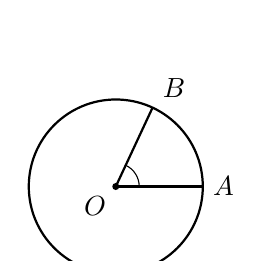
\begin{tikzpicture}[scale=0.85]
  \coordinate (O) at (0,0);
  \draw[thick] (O) circle (1.3);
  \coordinate (A) at (0:1.3);
  \coordinate (B) at (65:1.3);
  \draw[thick] (O) -- (A) node[right]{$A$};
  \draw[thick] (O) -- (B) node[above right]{$B$};
  \fill (O) circle (1.5pt) node[below left]{$O$};
  \draw (0.35,0) arc (0:65:0.35);
\end{tikzpicture}
\end{center}
\choice
{$\widehat{ABO}$}
{$\widehat{OMB}$}
{$\widehat{AMO}$}
{\True $\widehat{AOB}$}
\loigiai{
Góc ở tâm là góc có đỉnh trùng với tâm của đường tròn. Đỉnh $O$ là tâm của đường tròn và hai cạnh $OA, OB$ đi qua $A, B$ nên góc ở tâm là $\widehat{AOB}$.
}
\end{ex}

\begin{ex}
Trong các mệnh đề sau, mệnh đề nào đúng?
\choice
{Đường tròn chỉ có một trục đối xứng}
{Tâm đối xứng của đường tròn là mọi điểm trên đường tròn}
{\True Mọi đường kính của đường tròn đều là trục đối xứng của nó}
{Đường tròn không có trục đối xứng nào}
\loigiai{
Đường tròn là hình có vô số trục đối xứng, bất kỳ đường thẳng nào đi qua tâm (chứa đường kính) đều là một trục đối xứng của đường tròn đó.
}
\end{ex}

\begin{ex}
Một khúc sông rộng khoảng $250\text{ m}$. Một con đò chèo chéo qua sông bị dòng nước đẩy xiên nên phải chèo $320\text{ m}$ mới sang được bờ bên kia. Hỏi dòng nước đã đẩy chiếc đò lệch đi một góc xấp xỉ bằng bao nhiêu độ (góc giữa hướng vuông góc bờ sông và hướng chèo đò)?
\begin{center}
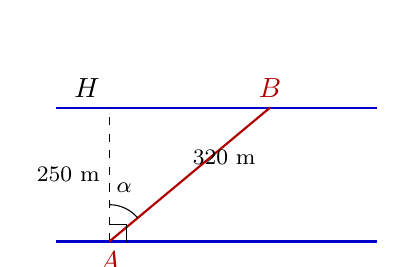
\begin{tikzpicture}[scale=0.85]
  \draw[thick, blue!80!black] (-0.8,0) -- (4,0);
  \draw[thick, blue!80!black] (-0.8,2) -- (4,2);
  \coordinate (A) at (0,0);
  \coordinate (H) at (0,2);
  \coordinate (B) at (2.4,2);
  \draw[dashed] (A) -- (H) node[above left]{$H$};
  \draw[thick, red!70!black] (A) node[below]{$A$} -- (B) node[above]{$B$};
  \draw (A) ++(0,0.25) -- ++(0.25,0) -- ++(0,-0.25);
  \draw (A) ++(0,0.55) arc (90:39.8:0.55);
  \node at (0.22,0.8) {\footnotesize $\alpha$};
  \node[left] at (0,1) {\footnotesize $250\text{ m}$};
  \node[above right] at (1.1,1) {\footnotesize $320\text{ m}$};
\end{tikzpicture}
\end{center}
\choice
{$25^\circ$}
{\True $39^\circ$}
{$45^\circ$}
{$51^\circ$}
\loigiai{
Gọi $\alpha$ là góc lệch giữa hướng chuyển động của đò và hướng vuông góc bờ sông. Ta có $\cos \alpha = \frac{250}{320} = 0{,}78125 \implies \alpha = \arccos(0{,}78125) \approx 38{,}62^\circ \approx 39^\circ$.
}
\end{ex}

\begin{ex}
Cho đường tròn $(O; 5\text{ cm})$ và một điểm $A$ nằm ngoài đường tròn sao cho $OA = 13\text{ cm}$. Qua $A$ kẻ tiếp tuyến $AB$ với đường tròn ($B$ là tiếp điểm). Độ dài đoạn thẳng $AB$ bằng:
\choice
{\True $12\text{ cm}$}
{$8\text{ cm}$}
{$\sqrt{194}\text{ cm}$}
{$18\text{ cm}$}
\loigiai{
Vì $AB$ là tiếp tuyến tại $B$ nên tam giác $OAB$ vuông tại $B$. Theo định lí Pythagore: $AB = \sqrt{OA^2 - OB^2} = \sqrt{13^2 - 5^2} = \sqrt{144} = 12\text{ cm}$.
}
\end{ex}


\newpage
\noindent\textbf{\large PHẦN II. CÂU TRẮC NGHIỆM ĐÚNG SAI}
\vspace{1mm}
\begin{ex}
Cho hai số thực $x, y$ thỏa mãn $x > y$. Xét tính Đúng/Sai của các khẳng định sau:
\choiceTF
{\True $x - 5 > y - 5$.}
{$-4x > -4y$.}
{\True $3x - 2 > 3y - 2$.}
{\True $-2x + 1 < -2y + 1$.}
\loigiai{
\begin{itemize}[leftmargin=*]
  \item a) Đúng. Trừ cả hai vế của bất đẳng thức $x > y$ với 5 thì giữ nguyên chiều: $x - 5 > y - 5$. Khẳng định Đúng.
  \item b) Sai. Nhân cả hai vế với số âm $-4$ thì phải đổi chiều: $-4x < -4y$. Khẳng định Sai.
  \item c) Đúng. Vì $x > y \implies 3x > 3y \implies 3x - 2 > 3y - 2$. Khẳng định Đúng.
  \item d) Đúng. Vì $x > y \implies -2x < -2y \implies -2x + 1 < -2y + 1$. Khẳng định Đúng.
\end{itemize}
}
\end{ex}

\begin{ex}
Cho tam giác $DEF$ vuông tại $D$, biết $DE = 5\text{ cm}$ và $DF = 12\text{ cm}$. Xét tính Đúng/Sai của các khẳng định sau:
\choiceTF
{\True Độ dài cạnh huyền $EF = 13\text{ cm}$.}
{$\sin E = \frac{5}{13}$.}
{\True $\cos F = \frac{12}{13}$.}
{$\tan E = \frac{5}{12}$.}
\loigiai{
\begin{itemize}[leftmargin=*]
  \item a) Đúng. Theo định lí Pythagore: $EF = \sqrt{DE^2 + DF^2} = \sqrt{5^2 + 12^2} = 13\text{ cm}$. Khẳng định Đúng.
  \item b) Sai. Ta có $\sin E = \frac{DF}{EF} = \frac{12}{13} \neq \frac{5}{13}$. Khẳng định Sai.
  \item c) Đúng. Ta có $\cos F = \frac{DF}{EF} = \frac{12}{13}$. Khẳng định Đúng.
  \item d) Sai. Ta có $\tan E = \frac{DF}{DE} = \frac{12}{5} \neq \frac{5}{12}$. Khẳng định Sai.
\end{itemize}
}
\end{ex}


\vspace{2mm}
\noindent\textbf{\large PHẦN III. CÂU TRẢ LỜI NGẮN}
\vspace{1mm}
\begin{ex}
Tìm $x$, biết: $\sqrt{2x - 1} = 3$.
\shortans{$x = 5$}
\loigiai{
Điều kiện xác định: $2x - 1 \ge 0 \iff x \ge \frac{1}{2}$.\par Bình phương hai vế: $2x - 1 = 9 \iff 2x = 10 \implies x = 5$ (thỏa mãn ĐKXĐ).
}
\end{ex}

\begin{ex}
Cho đường tròn $(O)$ có bán kính $R = 5\text{ cm}$. Khoảng cách từ tâm $O$ đến dây $AB$ bằng $3\text{ cm}$. Tính độ dài dây $AB$.
\shortans{$8\text{ cm}$}
\loigiai{
Kẻ $OH \perp AB$ tại $H$, suy ra $H$ là trung điểm của $AB$ và $OH = 3\text{ cm}$.\par Xét tam giác vuông $OAH$ vuông tại $H$: $AH = \sqrt{OA^2 - OH^2} = \sqrt{5^2 - 3^2} = 4\text{ cm}$.\par Độ dài dây $AB = 2 \cdot AH = 2 \cdot 4 = 8\text{ cm}$.
}
\end{ex}


\newpage
\noindent\textbf{\large PHẦN IV. TỰ LUẬN}
\vspace{1mm}
\noindent\textbf{Câu 1 (2,0 điểm).}

Giải các phương trình và bất phương trình sau:\par a) $(x - 3)(x - 4) = 0$.\par b) $\frac{x + 1}{x - 1} - \frac{x + 2}{x + 2} = \frac{6}{(x - 1)(x + 2)}$.\par c) $5x + 4 < 2x - 2$.\par d) $\frac{4x + 5}{2} - \frac{5x + 6}{3} \le 1$.

\noindent\textbf{Lời giải:}

a) $(x - 3)(x - 4) = 0 \iff x - 3 = 0$ hoặc $x - 4 = 0 \iff x = 3$ hoặc $x = 4$.\par Vậy tập nghiệm của phương trình là $S = \{3; 4\}$.\par b) Điều kiện xác định: $x \neq 1$ và $x \neq -2$.\par Ta có $\frac{x + 2}{x + 2} = 1$. Phương trình trở thành: $\frac{x + 1}{x - 1} - 1 = \frac{6}{(x - 1)(x + 2)}$\par $\iff \frac{(x + 1) - (x - 1)}{x - 1} = \frac{6}{(x - 1)(x + 2)} \iff \frac{2}{x - 1} = \frac{6}{(x - 1)(x + 2)}$\par $\iff 2(x + 2) = 6 \iff 2x + 4 = 6 \iff 2x = 2 \implies x = 1$ (không thỏa mãn ĐKXĐ).\par Vậy phương trình vô nghiệm.\par (Nếu đề bài là $\frac{x + 1}{x - 1} - \frac{x - 2}{x + 2} = \dots$ giải tương tự theo điều kiện).\par c) $5x + 4 < 2x - 2 \iff 5x - 2x < -2 - 4 \iff 3x < -6 \iff x < -2$.\par Vậy nghiệm của bất phương trình là $x < -2$.\par d) Quy đồng mẫu số chung là 6 và khử mẫu:\par $3(4x + 5) - 2(5x + 6) \le 6 \iff 12x + 15 - 10x - 12 \le 6$\par $\iff 2x + 3 \le 6 \iff 2x \le 3 \iff x \le \frac{3}{2}$.\par Vậy nghiệm của bất phương trình là $x \le \frac{3}{2}$.

\vspace{3mm}
\noindent\textbf{Câu 2 (1,0 điểm).}

Một người mua một cái bàn là và một cái quạt điện với tổng số tiền theo giá niêm yết là 750 nghìn đồng. Hiện tại cửa hàng đang thực hiện giảm giá $10\%$ đối với bàn là và $20\%$ đối với quạt điện so với giá niêm yết. Vì vậy người đó chỉ phải trả tổng cộng 625 nghìn đồng. Tính giá tiền một cái bàn là và một cái quạt điện theo giá niêm yết.

\noindent\textbf{Lời giải:}

Gọi giá niêm yết của bàn là và quạt điện lần lượt là $x$ và $y$ (nghìn đồng; $0 < x, y < 750$).\par Tổng giá niêm yết là 750 nghìn đồng: $x + y = 750 \quad (1)$.\par Giá bàn là sau khi giảm $10\%$ là $(1 - 0{,}1)x = 0{,}9x$ nghìn đồng.\par Giá quạt điện sau khi giảm $20\%$ là $(1 - 0{,}2)y = 0{,}8y$ nghìn đồng.\par Tổng số tiền thực tế phải trả là 625 nghìn đồng: $0{,}9x + 0{,}8y = 625 \quad (2)$.\par Từ (1) và (2) ta có hệ phương trình: $\begin{cases} x + y = 750 \\ 0{,}9x + 0{,}8y = 625 \end{cases}$\par Nhân hai vế phương trình đầu với 0,8: $\begin{cases} 0{,}8x + 0{,}8y = 600 \\ 0{,}9x + 0{,}8y = 625 \end{cases}$\par Trừ vế theo vế: $0{,}1x = 25 \implies x = 250$ (thỏa mãn).\par Suy ra $y = 750 - 250 = 500$ (thỏa mãn).\par Vậy giá niêm yết của bàn là là 250 nghìn đồng và của quạt điện là 500 nghìn đồng.

\vspace{3mm}
\newpage
\noindent\textbf{Câu 3 (0,5 điểm).}

Cho tam giác $ABC$ vuông tại $A$ có $\widehat{C} = 30^\circ$, cạnh $AB = 8\text{ cm}$. Tính:\par a) Số đo góc $B$.\par b) Độ dài các cạnh $AC$ và $BC$.

\noindent\textbf{Lời giải:}

a) Trong tam giác $ABC$ vuông tại $A$:\par $\widehat{B} = 90^\circ - \widehat{C} = 90^\circ - 30^\circ = 60^\circ$.\par b) Áp dụng tỉ số lượng giác của góc nhọn trong tam giác vuông $ABC$:\par Cạnh huyền $BC = \frac{AB}{\sin C} = \frac{8}{\sin 30^\circ} = \frac{8}{0{,}5} = 16\text{ cm}$.\par Cạnh góc vuông $AC = AB \cdot \cot C = 8 \cdot \cot 30^\circ = 8\sqrt{3} \approx 13{,}86\text{ cm}$.

\vspace{3mm}
\noindent\textbf{Câu 4 (0,5 điểm).}

Cho tam giác $ABC$ vuông tại $A$, đường cao $AH$. Chứng minh rằng $AH \cdot BC = AB \cdot AC$.

\noindent\textbf{Lời giải:}

Xét hai tam giác vuông $\Delta AHB$ và $\Delta CAB$ có:\par - $\widehat{AHB} = \widehat{CAB} = 90^\circ$.\par - Góc $\widehat{B}$ chung.\par Suy ra $\Delta AHB \backsim \Delta CAB$ (g-g).\par Do đó ta có tỉ số đồng dạng giữa các cạnh tương ứng:\par $\frac{AH}{CA} = \frac{AB}{CB} \implies AH \cdot BC = AB \cdot AC$ (đpcm).

\vspace{3mm}

\vfill
\begin{center}
  \textbf{--- HẾT ---}
\end{center}
\end{document}
